Our definition of incidence geometry is a kind of \textbf{theory}, and a theory is only really useful if it has at least one \textbf{model}.
So before we develop our theory of geometry further let's take a moment to construct some models.
Remember that the words ``point'', ``collinear'', and ``line'' are context-dependent -- what they mean depends on the model -- and so we may end up using these words in unintuitive ways.



\subsection{The Cartesian Plane and Friends}

We'll start with a model of incidence geometry with which you are probably already familiar: the cartesian plane.
To define this or any model it's enough to specify (1) what our points are and (2) what it means for three points to be collinear.
At risk of giving away the punchline, in this model points are pairs of numbers and lines are what you expect.

\begin{prop}[Cartesian Plane] \label{prop:rr2-incidence-geo}
Define a ternary relation on \(\RR^2\) as follows.
Given \(A = (a_x, a_y)\), \(B = (b_x, b_y)\), and \(C = (c_x, c_y)\) in \(\RR^2\), we say that \(\COLLINEAR{A}{B}{C}\) if and only if \(A\), \(B\), and \(C\) are not all equal and \[ \DET \begin{bmatrix} a_x & a_y & 1 \\ b_x & b_y & 1 \\ c_x & c_y & 1 \end{bmatrix} = 0. \]
This relation makes the set \(\RR^2\) an incidence geometry, which we call the \emph{cartesian plane}\index{cartesian plane}.
\end{prop}

\begin{proof}
IG1, IG2, and IG3 can be verified directly, and we can see that IG4 holds by considering the points \((0,0)\), \((0,1)\), and \((1,0)\).
So it suffices to show that IG5 holds.
To this end suppose we have \(A\), \(B\), \(U\), and \(V\).
Expanding and rearranging the known determinants, we have \[ (b_x - a_x)(u_y - a_y) = (b_y - a_y)(u_x - a_x) \] and \[ (b_x - a_x)(v_y - a_y) = (b_y - a_y)(v_x - a_x). \]
If \(a_x = b_x\), then we see that \(u_x = a_x = v_x\) and thus \(\COLLINEAR{A}{U}{V}\).
Similarly, if \(a_y = b_y\), we see that \(u_y = a_y = v_y\) and so \(\COLLINEAR{A}{U}{V}\).
Finally, suppose we have \(a_x \neq b_x\) and \(a_y \neq b_y\).
Now we have \[ \frac{u_y - a_y}{u_x - a_x} = \frac{b_y - a_y}{b_x - a_x} = \frac{v_y - a_y}{v_x - a_x}. \]
Equating the first and last of these expressions we see that \(\COLLINEAR{A}{U}{V}\).
\end{proof}

This might seem like a strange way to define ``collinearity'', but it is easy to compute, and by expanding the determinant we can see that the lines in this geometry are precisely the solutions of linear equations.

\begin{cor}[Lines in \(\RR^2\)] \label{cor:cartesian-lines}
Let \(A = (a_x, a_y)\) and \(B = (b_x, b_y)\) be distinct cartesian points.
Then \(\LINE{A}{B}\) is the set of all points \(X = (x,y)\) which satisfy the equation \[ (b_y-a_y)x - (b_x-a_x)y + a_yb_x - a_xb_y = 0. \]
\end{cor}

That equation may look familiar as the standard form equation of a line.
You might have noticed that our proof of \ref{prop:rr2-incidence-geo} used nothing more than the arithmetic on \(\RR\).
This means that the result still holds if we replace \(\RR\) by any object \(F\) where we have an arithmetic which behaves like that of \(\RR\).
Such objects are called \emph{fields}, and there are many examples, including the field \(\QQ\) of rational numbers and the field \(\CC\) of complex numbers.
So we immediately get some additional models as well.

\begin{cor}
The sets \(\QQ^2\) and \(\CC^2\) are incidence geometries, which we call the \emph{rational plane} and the \emph{complex plane}, respectively.
\end{cor}

Note that lines in \(\QQ^2\) look much like lines in \(\RR^2\) except that they are filled with ``holes''; any point on a line in \(\RR^2\) which has an irrational coordinate is not on the corresponding line in \(\QQ^2\).
Lines in \(\CC^2\) are stranger still.



\subsection{The Unit Disc}

Once we have an incidence geometry \(P\) lying around, one way to try to build new ones is by restricting the collinearity on \(P\) to subsets of \(P\).

\begin{prop}[Unit Disc]
Let \(\mathbb{D} = \{ (x,y) \in \RR^2 \mid x^2 + y^2 < 1 \}\); these are points in the cartesian plane which are inside the unit circle.
Given points \(A\), \(B\), and \(C\) in \(\mathbb{D}\), we say they are collinear in \(\mathbb{D}\) if they are collinear in \(\RR^2\).
This relation makes \(\mathbb{D}\) an incidence geometry which we call the \emph{Unit Disc}.
\end{prop}

Lines in the unit disc are chords of the unit circle (not including their endpoints).
Already the word ``line'' is being twisted.



\subsection{The Fano Plane}

We will now see a very different and somewhat strange model of incidence geometry.

\begin{dfn}[The Fano Plane]
Let \(P = \{1,2,3,4,5,6,7\}\), and then let \(L = \{\{1,2,3\},\) \(\{2,4,6\},\) \(\{1,4,7\},\) \(\{1,5,6\},\) \(\{2,5,7\},\) \(\{3,4,5\},\) \(\{3,6,7\}\}\).
We then define a ternary relation on \(P\) by \(\COLLINEAR{a}{b}{c}\) if and only if \(\{a,b,c\}\) is not a singleton and is contained in some \(\ell \in L\).
The set \(P\) with this ternary relation is called the \emph{Fano Plane}.
\end{dfn}

It turns out that the Fano plane is an incidence geometry.



\subsection{The Antipodal Sphere}

Our next example is especially weird.

\begin{prop}[Antipodal Sphere]
Let \(S = \{ (x,y,z) \in \RR^3 \mid x^2 + y^2 + z^2 = 1 \}\), and consider the equivalence relation \(\sigma\) on \(S\) such that \(x \,\sigma\, y\) if and only if \(y = \pm x\).
We define the set \(\mathbb{A} = S/\sigma\), and call the elements of \(\mathbb{A}\) \emph{antipodal pairs}.
We define a ternary relation on \(\mathbb{A}\) by \(\COLLINEAR{A}{B}{C}\) if and only if \[ \DET \begin{bmatrix} a_x & a_y & a_z \\ b_x & b_y & b_z \\ c_x & c_y & c_z \end{bmatrix} = 0. \] This relation is well-defined, and makes \(\mathbb{A}\) an incidence geometry which we call the \emph{antipodal sphere}.
\end{prop}

Before we approach this proof, notice that the ``points'' in this model are actually \emph{pairs} of ``points'' in \(\RR^3\).
Specifically, each point in \(\mathbb{A}\) is a set of the form \( \{ (\alpha, \beta, \gamma), (-\alpha, -\beta, -\gamma) \} \) for some real numbers \(\alpha, \beta, \gamma\) with \(\alpha^2 + \beta^2 + \gamma^2 = 1\).
Such pairs of points are called \emph{antipodes}.
We can think of these ``points'' as the intersection of the unit sphere with a line through the origin; see \autoref{fig:antipodal-sphere-point} for a picture.

\begin{figure}
\begin{center}
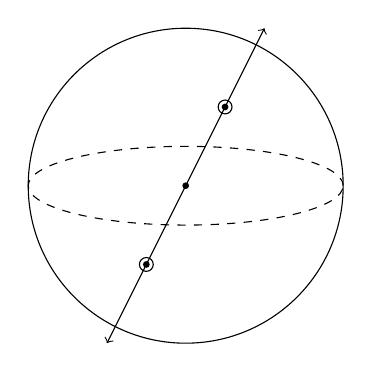
\begin{tikzpicture}[scale=0.5]
  \draw (0,0) circle (4);
  \draw [dashed] (0,0) ellipse (4 and 1);
  \draw [fill] (0,0) circle [radius=2pt];
  \draw [fill] (1,2) circle [radius=2pt];
  \draw [fill] (-1,-2) circle [radius=2pt];
  \draw (1,2) circle [radius=5pt];
  \draw (-1,-2) circle [radius=5pt];
  \draw [<->] (2,4) -- (-2,-4);
\end{tikzpicture}
\caption{\label{fig:antipodal-sphere-point}A ``point'' in the antipodal sphere (circled).}
\end{center}
\end{figure}



\subsection{The Hyperbolic Half-Plane}

We will now construct a strange model of incidence geometry.
For this example, our set of points is \(\mathbb{H} = \{ (x,y) \mid x,y \in \RR\ \mathrm{and}\ y > 0 \}\).
Suppose we have two points \(A = (a_x, a_y)\) and \(B = (b_x, b_y)\).
If \(a_x \neq b_x\), then the \emph{ideal point} of \(A\) and \(B\) is the number \[ I_{A,B} = \frac{b_x^2 + b_y^2 - a_x^2 - a_y^2}{2(b_x - a_x)}. \]
Intuitively, the ideal point is the \(x\)-coordinate of the point on the cartesian \(x\)-axis which is ``equidistant'' from \(A\) and \(B\).
More important for us is the following property of the ideal point.

\begin{lem}
Let \(A = (a_x, a_y)\) and \(B = (b_x, b_y)\) be points in \(\mathbb{H}\) such that \(a_x \neq b_x\).
Then the ideal point \(I_{A,B}\) of \(A\) and \(B\) is the unique solution \(X\) of the following equation.
\[ (a_x - X)^2 + a_y^2 = (b_x - X)^2 + b_y^2. \]
\end{lem}

We use the ideal point to define a collinearity relation on \(\mathbb{H}\) as follows.

\begin{prop}\label{prop:hyp-half-plane}
Define a ternary relation \(\COLLINEAR{\ast}{\ast}{\ast}\) on \(\mathbb{H}\) as follows.
Given points \(A = (a_x, a_y)\), \(B = (b_x, b_y)\), and \(C = (c_x, c_y)\) in \(\mathbb{H}\), we say that \(\COLLINEAR{A}{B}{C}\) if \(A\), \(B\), and \(C\) are not all equal and one of the following holds.
\begin{proplist}
\item \(a_x = b_x\) and \(a_y = b_y\)
\item \(a_x = b_x\) and \(a_y \neq b_y\) and \(c_x = a_x\).
\item \(a_x \neq b_x\) and \[ (c_x - I_{A,B})^2 + c_y^2 = (a_x - I_{A,B})^2 + a_y^2. \]
\end{proplist}
This relation makes \(\mathbb{H}\) an incidence geometry, which we call the \emph{hyperbolic half-plane}\index{hyperbolic half-plane}.
\end{prop}

\begin{proof}
Note that IG3 holds by definition. (@@@)
\end{proof}

We can show that the lines in this incidence geometry come in two flavors, which we will call the Type I and Type II lines.

\begin{cor}[Lines in \(\mathbb{H}\)]
Let \(A, B \in \mathbb{H}\) be distinct points.
\begin{proplist}
\item If \(a_x = b_x\) we say \(\LINE{A}{B}\) is of \emph{Type I}, and we have \[ \LINE{A}{B} = \{ (x,y) \in \mathbb{H} \mid x = a_x \}. \]
\item If \(a_x \neq b_x\) we say \(\LINE{A}{B}\) is of \emph{Type II}, and we have \[ \LINE{A}{B} = \{ (x,y) \in \mathbb{H} \mid (x - I_{A,B})^2 + y^2 = (a_x - I_{A,B})^2 + a_y^2 \}. \]
\end{proplist}
\end{cor}

Viewed as sets in the cartesian plane, the Type I lines in \(\mathbb{H}\) are vertical half lines, and the Type II lines in \(\mathbb{H}\) are semicircles centered on the \(x\)-axis.
In fact the cartesian center of a Type II line is the point \((I_{A,B},0)\).

\begin{figure}[h]
\begin{center}
\begin{tikzpicture}
  \draw [dashed,<->] (-3,0) -- (3,0);
  \draw [->] (-2,0) -- (-2,3);
  \draw (2,0) arc (0:180:1.5);
  \node at (-3,1) {Type I};
  \node at (3,1) {Type II};
\end{tikzpicture}
\caption{\label{fig:lines-in-hyp-half-plane}Lines in \(\mathbb{H}\).}
\end{center}
\end{figure}



%---------%
\Exercises%
%---------%

\begin{exercise}[A parallel criterion in \(\RR^2\).] \label{exerc:parallels-in-rr2}
Let \(A = (a_1,a_2)\), \(B = (b_1,b_2)\), \(C = (c_1,c_2)\), and \(D = (d_1,d_2)\) be points in the cartesian plane with \(A \neq B\) and \(C \neq D\).
Show that \(\LINE{A}{B}\) and \(\LINE{C}{D}\) are parallel if and only if \[ \DET \begin{bmatrix} b_1 - a_1 & d_1 - c_1 \\ b_2 - a_2 & d_2 - c_2 \end{bmatrix} = 0. \]
\end{exercise}


\begin{exercise}[A collinearity criterion in \(\RR^2\).]
Let \(A = (a_x,a_y)\), \(B = (b_x,b_y)\), and \(C = (c_x,c_y)\) be points in \(\RR^2\) such that \(A \neq C\) and \(B \neq C\).
Show that \(A\), \(B\), and \(C\) are collinear if and only if \[ \DET \begin{bmatrix} a_x - c_x & b_x - c_x \\ a_y - c_y & b_y - c_y \end{bmatrix} = 0. \]
\end{exercise}


\begin{exercise}
Complete the proof of \propref{prop:hyp-half-plane}.
\end{exercise}
